%% REPLACE sXXXXXXX with your student number
\def\studentNumber{s2178120}


%% START of YOUR ANSWERS
%% Add answers to the questions below, by replacing the text inside the brackets {} for \youranswer{ "Text to be replaced with your answer." }. 
%
% Do not delete the commands for adding figures and tables. Instead fill in the missing values with your experiment results, and replace the images with your own respective figures.
%
% You can generally delete the placeholder text, such as for example the text "Question Figure 3 - Replace the images ..." 
%
% There are 5 TEXT QUESTIONS. Replace the text inside the brackets of the command \youranswer with your answer to the question.
%
% There are also 3 "questions" to replace some placeholder FIGURES with your own, and 1 "question" asking you to fill in the missing entries in the TABLE provided. 
%
% NOTE! that questions are ordered by the order of appearance of their answers in the text, and not necessarily by the order you should tackle them. You should attempt to fill in the TABLE and FIGURES before discussing the results presented there. 
%
% NOTE! If for some reason you do not manage to produce results for some FIGURES and the TABLE, then you can get partial marks by discussing your expectations of the results in the relevant TEXT QUESTIONS. The TABLE specifically has enough information in it already for you to draw meaningful conclusions.
%
% Please refer to the coursework specification for more details.


%% - - - - - - - - - - - - TEXT QUESTIONS - - - - - - - - - - - - 

%% Question 1:
\newcommand{\questionOne} {
\youranswer{We can see from Figure 1 that VGG08 model achieves a high accuracy and its loss descends by epoch, while VGG38 has an accuracy close to 0, and its loss does not descend. In Figure 2 and 3, the average gradients of VGG08 are in a reasonable scale, while the gradients of VGG38 are too small that the model cannot be trained by back propagation, thus suffers from VGP.}
}

%% Question 2:
\newcommand{\questionTwo} {
\youranswer{
Suppose we set the batch size of the model to $m$. The following analysis is the same for training and test phase.

For a particular batch, we calculate the mean and variance of the batch B, denoted as
\begin{equation}
    \label{eq.bn_mean_var}
    \mu_B=\frac{1}{m}\sum_{i=1}^{m}x_i,\ and\  \sigma_B^2=\frac{1}{m}\sum_{i=1}^{m}(x_i-\mu_B)^2
\end{equation}
where $m$ is the batch size. For each $d$-dimensional input $x=(x^{(1)},x^{(2)},\dots,x^{(d})$, we normalize it as
\begin{equation}
    \label{eq.bn}
    \hat{x}_i^{(k}=\frac{x_i^{(k)}-\mu_B^{(k)}}{\sqrt{{\sigma_B^{(k)}}^2+\epsilon}}
\end{equation}
where $k\in [1, d]$ is the dimension and $i\in [1,m]$.
In Batch Norm, we restrict each dimension of each data within $[-1,1]$. Since $z=\sigma(w^T x+b)$ and $\frac{\partial z}{\partial  x}=w\frac{\partial z}{\partial \sigma}$, when x is restricted to a range, then $w$ can not be too large or too small (otherwise $z$ will be very different to the ground truth), so the gradient of $w$ will not be too large or too small, thus overcome the VGP in deep CNN. 
}
}

%% Question 3:
\newcommand{\questionThree} {
\youranswer{A simple way to express residual connection is
\begin{equation}
    x_L=F(x_l)+x_l
\end{equation}
where $F(x_l)$ is the output of a block with $x_l$ as input. If the loss is $L$, then the gradient is
\begin{equation}
    \frac{\partial L}{\partial x_l}=\frac{\partial L}{\partial x_L}\frac{\partial x_L}{\partial x_l}=\frac{\partial L}{\partial x_L}(\frac{\partial F}{\partial x_l}+I)
\end{equation}
where $I$ is the identity matrix. The result shows that the gradient of $x_l$ is not smaller than the gradient of $x_L$, which reduces the VGP problem.
}
}

%% Question 4:
\newcommand{\questionFour} {
\youranswer{The experiment results of the models are shown in Table~\ref{tab:CIFAR_results}. We can see that, VGG38 BN + RC with LR = 1e-2 achieves the best performance, which shows that BatchNorm and residual connection do help to boost the performance. It also implies that the combination of BatchNorm and residual connections is better than the parts. We can see that VGG38 BN beats VGG0, which indicates the contribution of BatchNorm in overcoming the VGP. The comparison between VGG38 BN and VGG38 RC shows that residual connection is more important to overcoming VGP than BatchNorm. We can also see that a higher learning rate leads to a better performance in our setting, which means that VGG38 model with LR = 1e-3 may suffers from underfitting. 

The training and validation curves for the best model is shown in Figure~\ref{fig:acc_cur_bestModel}. We can see that with BatchNorm and residual connections, the model converges faster and reaches a higher accuracy for both training and validation dataset. We can conclude that BatchNorm and residual connections can overcome VGP and help the model to converge.

The gradient flow of the best model is shown in Figure~\ref{fig:grad_flow_bestModel}. The average gradient of VGG38 BN+RC is significantly greater than the gradients of VGG38 which has no BatchNorm and residual connections. This result implies that BatchNorm and residual connections can directly overcome VGP.

Further experiments can be done. Firstly, the size of the residual block is not sufficiently explored in this work. Second, the architecture of the model is fixed in our experiments, we can test BatchNorm and residual connections on many more different architectures.

The behaviour of BN and RC is not clear enough. To go a step further, we can analyze exactly how much the residual connections and BatchNorm contributes to each layer compared to the original architecture.
}
}

%% Question 5:
\newcommand{\questionFive} {
\youranswer{In this work, we compare the performance of VGG08 and VGG38 models and observes the VGP, as well as the visualization of the gradient flow. To overcome VGP, we apply Batch Normalization~\cite{ioffe2015batch} and Residual Connections~\cite{he2016deep} on VGG38 and achieves a higher performance than VGG08. The theoretical analysis is also proposed. There remains questions to answer, such as the behaviour of BN and RC, and the performance of more architectures with BN and RC applied.
}
}

%% - - - - - - - - - - - - FIGURES - - - - - - - - - - - - 

%% Question Figure 3:
\newcommand{\questionFigureThree} {
\youranswer{
\begin{figure}[t]
    \centering
    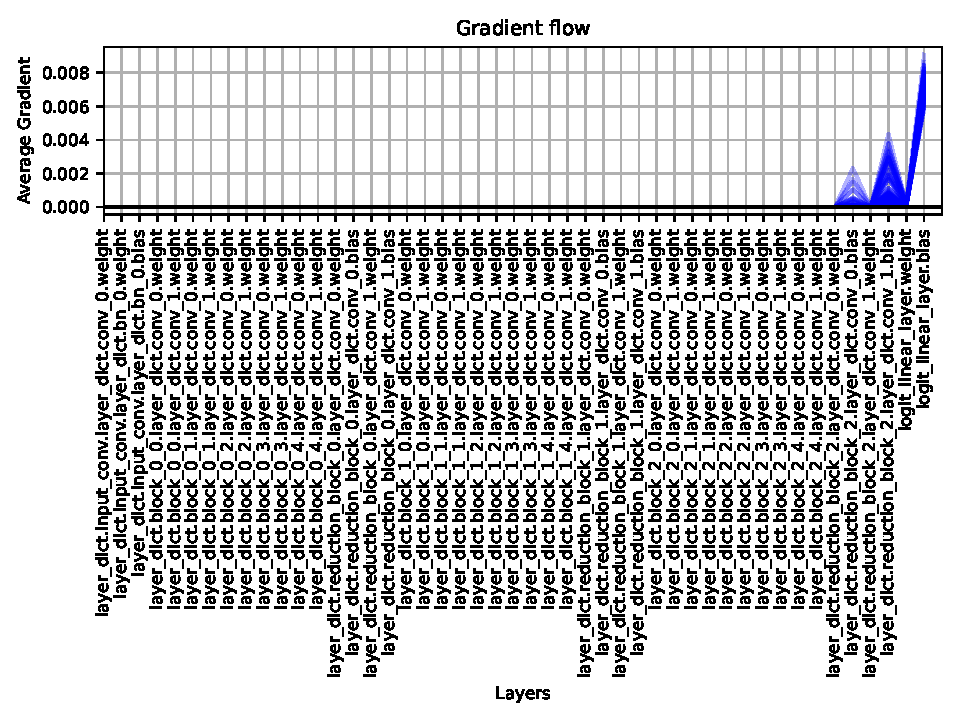
\includegraphics[width=\linewidth]{figures/grad_flow_vgg38.pdf}
    \caption{Gradient Flow on VGG38}
    \label{fig:grad_flow_38}
\end{figure}
}
}

%% Question Figure 4:
\newcommand{\questionFigureFour} {
\youranswer{
\begin{figure}[t]
    \centering
    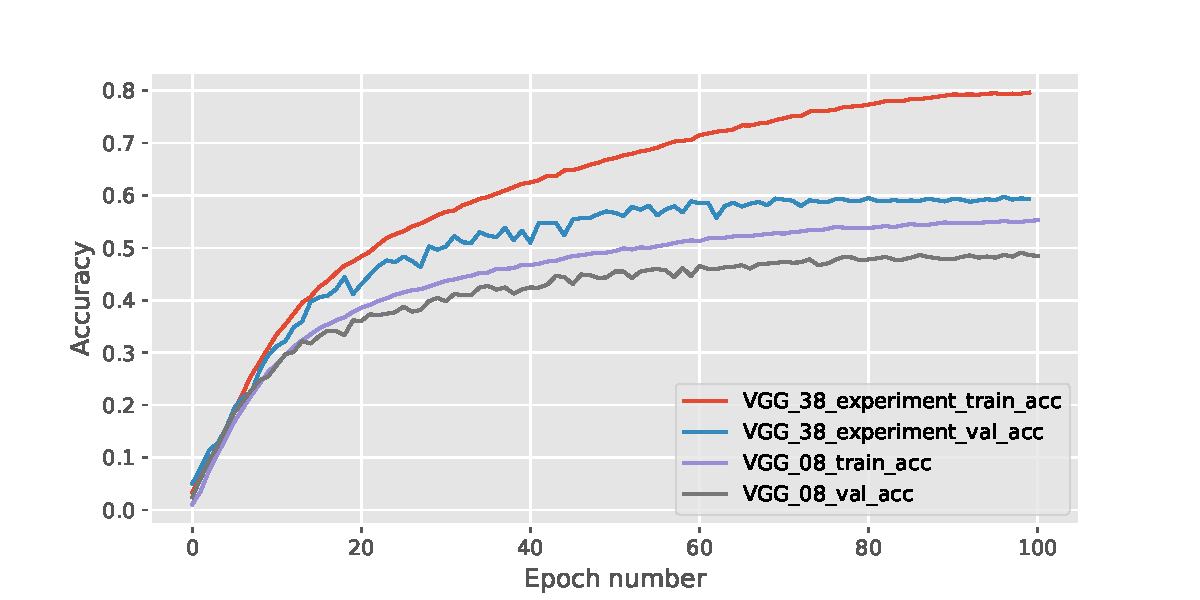
\includegraphics[width=\linewidth]{figures/bn_rc_38_accuracy_performance.pdf}
    \caption{Training curves for VGG38 BN + RC}
    \label{fig:acc_curve_bestModel}
\end{figure}
}
}

%% Question Figure 5:
\newcommand{\questionFigureFive} {
\youranswer{
\begin{figure}[t]
    \centering
    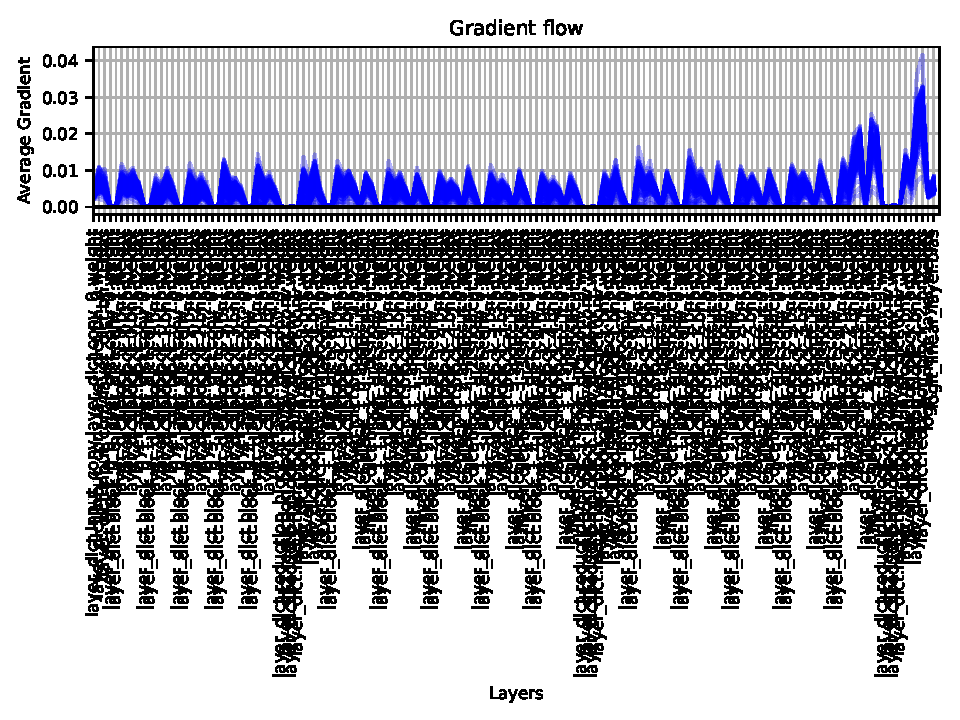
\includegraphics[width=\linewidth]{figures/grad_flow_vgg38_bnrc.pdf}
    \caption{Gradient Flow on VGG38 BN + RC}
    \label{fig:grad_flow_bestModel}
\end{figure}
}
}

%% - - - - - - - - - - - - TABLES - - - - - - - - - - - - 

%% Question Table 1:
\newcommand{\questionTableOne} {
\youranswer{
\begin{table*}[t]
    \centering
    \begin{tabular}{lr|ccccc}
    \toprule
        Model                   & LR   & \# Params & Train loss & Train acc & Val loss & Val acc \\
    \midrule
        VGG08                   & 1e-3 & 60 K      &  1.74      & 51.59     & 1.95     & 46.84 \\
        VGG38                   & 1e-3 & 336 K     &  4.61      & 00.01     & 4.61     & 00.01 \\
        VGG38 BN                & 1e-3 & 339 K     &  1.51      & 56.92     & 1.99     & 47.48 \\
        VGG38 RC                & 1e-3 & 336 K     &  1.33      & 61.52     & 1.84     & 52.32 \\
        VGG38 BN + RC           & 1e-3 & 339 K     &  1.26      & 62.99     & 1.73     & 53.76 \\
        VGG38 BN                & 1e-2 & 339 K     &  1.70      & 52.28     & 1.99     & 46.72 \\
        VGG38 BN + RC           & 1e-2 & 339 K     &  0.77      & 76.63     & 1.70     & 59.72 \\
    \bottomrule
    \end{tabular}
    \caption{Experiment results (number of model parameters, Training and Validation loss and accuracy) for different combinations of VGG08, VGG38, Batch Normalisation (BN), and Residual Connections (RC), LR is learning rate.}
    \label{tab:CIFAR_results}
\end{table*} 
}
}

%% END of YOUR ANSWERS